\section{Different Scenarios} 

Different size and coverage scenarios were explored to analyse the relationship ordering. 

One thousand simulations were run for each scenario. There was no set seed for sample size scenarios to allow for variability. 

Each scenario used a default threshold of 0.9, odds ratio of 1.5, and analysed 100 SNPs. This is to follow the basic scientific principle to only change one variable at a time while holding the rest as controls. All covariate values are explicitly specified for each set of simulations for clarity and confidence intervals are recorded as 95\% CIs. 

Scales have been adjusted per each simulation on purpose, so trends may be easily identified. All specific values from simulation outputs can be found in tables in the Appendix. 






%ORDERED VS NOT ORDERED 
\subsection{Ordered vs. Not Ordered}
\subsubsection{Size and Ordering}
Analysis of how ordering effects size was considered. A threshold of 0.9, odds ratio of 1.5, and 100 SNPs was used. Simulation results support fundamental and intuitive understanding that ordering reduces the credible set size. Ordered sets had on average 4.4\% smaller size  (3.7\% to 5.2\%). 

%Ordered_Size Boxplot
\begin{figure}[H]
\centering
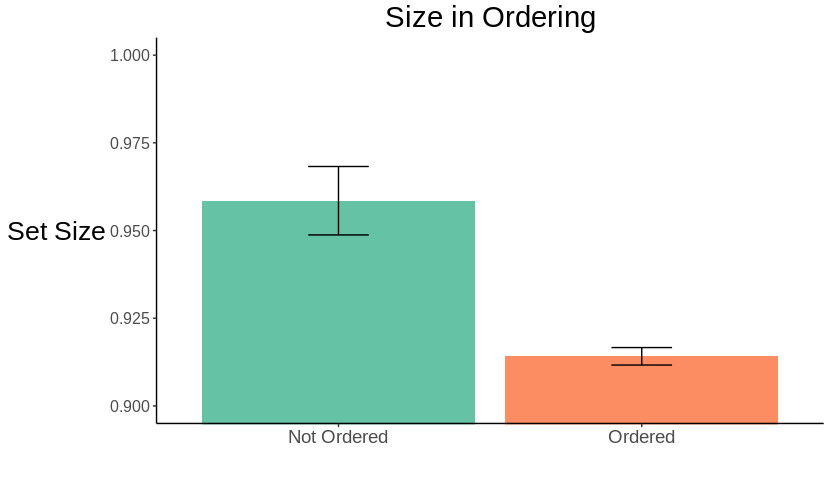
\includegraphics[scale=0.625]{images/Barplots/Ordered_Size.png}
\caption{Ordered vs. Not Ordered Size}
    \smallskip
    \footnotesize
Figure created from covariate values of: 1000 simulations, threshold of 0.9, odds ratio of 1.5, sample size of 1000 cases and 1000 controls, and 100 SNPs. 
\label{fig: Ordered_Size}
\end{figure}

\subsubsection{Coverage and Ordering}
Next, we wanted to consider how coverage changed when accounting for ordering credible sets. Simulation results showed coverage is higher in ordered sets compared to not ordered sets, after controlling for odds ratio (1.5), threshold (0.9), and sample size N cases(1000) and N controls (1000). 

The simulation proves that coverage is effected by ordering. This means that when data are ordered, it introduces information about containing the causal variant, outside of the sum of posterior probabilities. We will refer to this as overcoverage, where the specified value for a threshold is exceeded due to additional information introduced from ordering the sets. Coverage was 4\% greater in ordered sets (4.8\% to 3.2\%). 

%Ordered_Cov Boxplot
\begin{figure}[H]
\centering
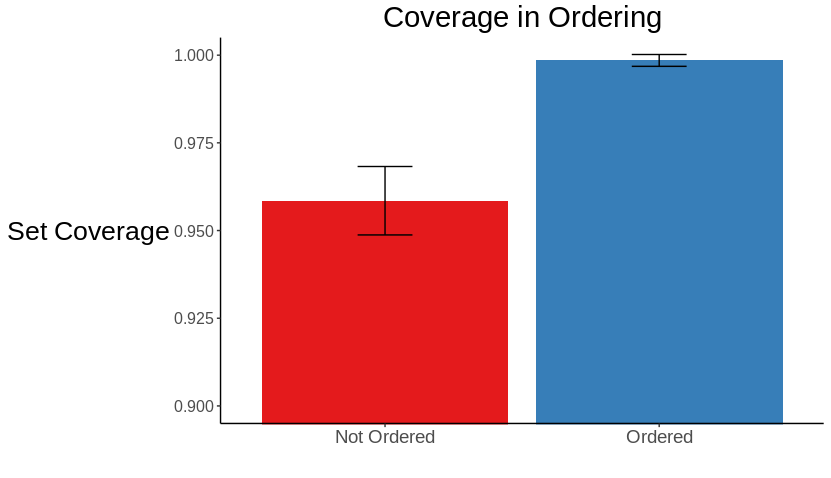
\includegraphics[scale=0.625]{images/Barplots/Ordered_Cov.png}
\caption{Ordered vs. Not Ordered Coverage}
    \smallskip
    \footnotesize
Figure created from covariate values of: 1000 simulations, threshold of 0.9, odds ratio of 1.5, sample size of 1000 cases and 1000 controls, and 100 SNPs. 
\label{fig: Ordered_Cov}
\end{figure}

%ODDS RATIOS
\subsection{Odds Ratios}

Odds ratios represent the effect size ($\Theta$) that a SNP has on the association of the phenotype. The larger the odds ratio, the stronger the signal, and therefore more confident inference for which variant is causal. Odds ratios were explored within a sensible range of 1.00 to 1.5. For all odds ratios simulations, the threshold was 0.9, sample size of 1000 cases and 1000 controls, and 100 SNPs. 


\subsubsection{Odds Ratios and Size}
Across all odds ratio values the average size of the credible set was reduced when ordering. Sets that were not ordered, were much larger for OR = 1.5. Where the signal for that variant is very strong, and has a much high posterior probability compared to other OR values.


\begin{figure}[H]
\centering
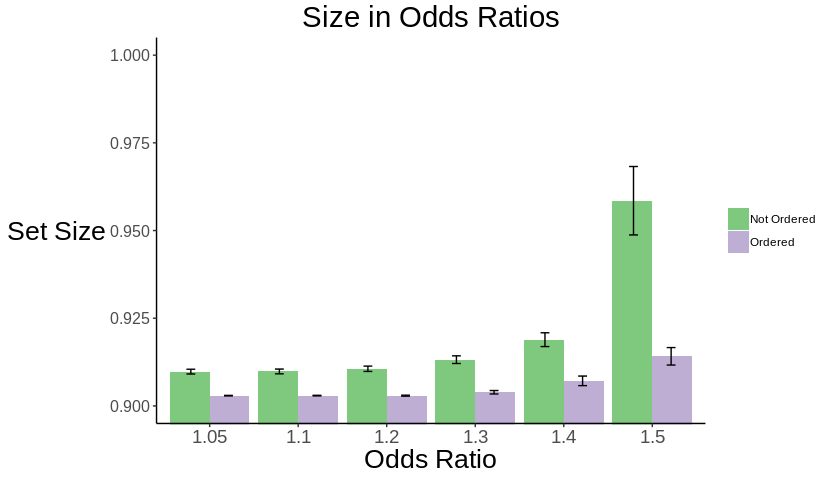
\includegraphics[scale=0.625]{images/Barplots/OR_Size.png}
\caption{Odds Ratios and Size}
\label{fig: OR_Size}
\end{figure}

\subsubsection{Odds Ratios and Coverage}
The trend between varying odds ratios and coverage did not show consistent overcoverage as was hypothesised. An odds ratio of 1.0 was considered, since it represents that no SNP has any effect on phenotype. Theoretically if ordering had no effect, the coverage would be the same for ordered versus not ordered sets. However, in low odds ratios 1.0-1.1, it was found that ordering the sets 


\begin{figure}[H]
\centering
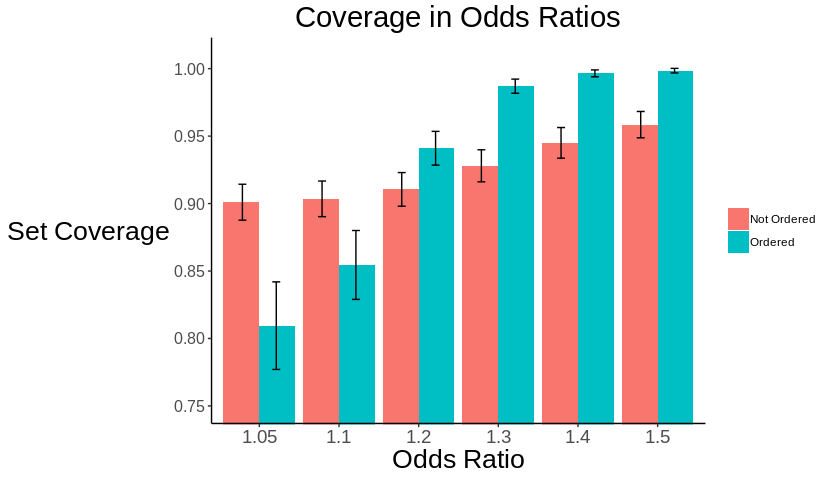
\includegraphics[scale=0.625]{images/Barplots/OR_Cov.png}
\caption{Odds Ratios and Size}
\label{fig: OR_Size}
\end{figure}

The trend in coverage over different values of odds ratios 


%THRESHOLDS 
\subsection{Thresholds}
Different threshold levels were investigated where threshold was set at 0.5, 0.9, and 0.99. Controlled variables were OR (1.5) and 
sample size N cases (1000) and N controls. 

Ordering reduced set sizes across all thresholds. Average difference in size and variance is greater in lower thresholds than higher thresholds.

\begin{figure}[H]
\centering
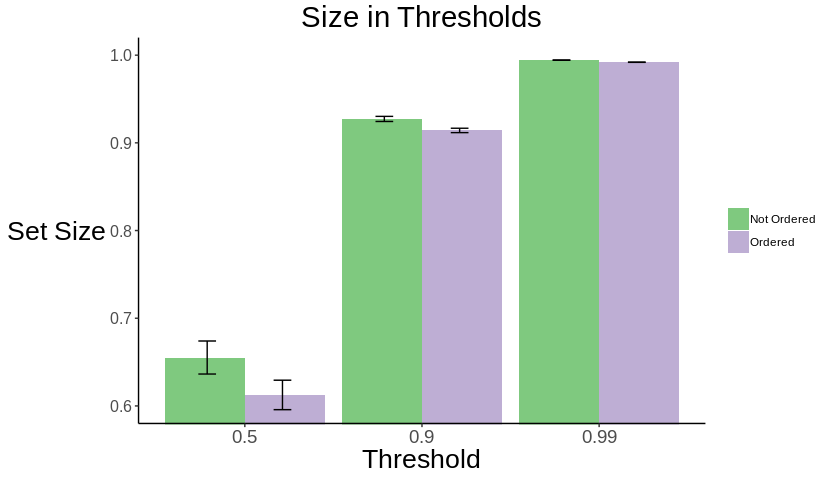
\includegraphics[scale=0.625]{images/Barplots/Thr_Size.png}
\caption{Thresholds and Size}
\label{fig: Thr_Size}
\end{figure}

Coverage was analysed across different thresholds. Simulations revealed overcoverage in ordered sets at the 0.5 and 0.9 level. \hl{At the 0.9 level the ordered coverage upper confidence interval was marginally over one, an unreal result. However, at the 0.99 level the not ordered coverage upper confidence interval returned an unreal result over one.}

Overcoverage for threshold=0.5 was 23.3\% (24.8\% to 21.8\%); threshold 0.9= 4.0\% (4.8\% to 3.2\%). threshold=0.99 0.05\% (1.5\% to -0.0048\%)

\begin{figure}[H]
\centering
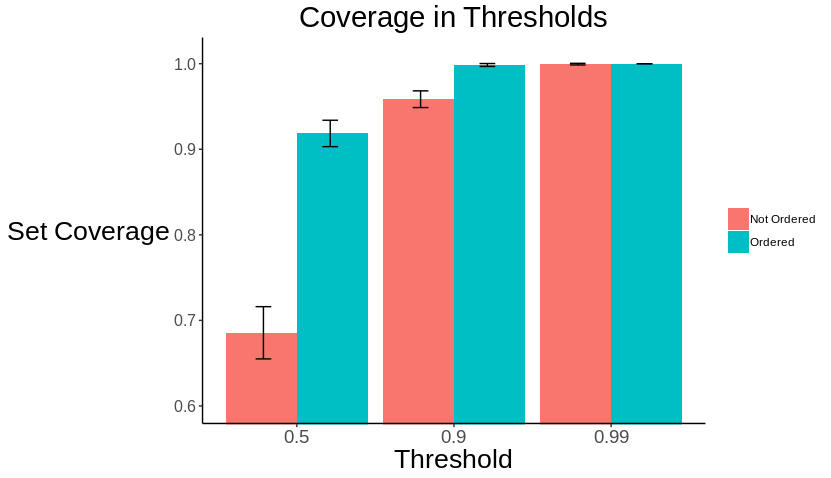
\includegraphics[scale=0.625]{images/Barplots/Thr_Cov.png}
\caption{Thresholds and Coverage}
\label{Thr_Cov}
\end{figure}


%SAMPLE SIZE 
\subsection{Sampling Size (n)}


Different scenarios of sampling were simulated. The ratio of cases and controls was kept the same where s=0.5 throughout the different sampling numbers tested. The sample sizes tested were 1000, 5000, 10000.  \hl{There was no seed used in sample size simulations to allow for variability. For this reason, the sample size of 5000 has more variability - not really sure about this.}

\begin{figure}[H]
\centering
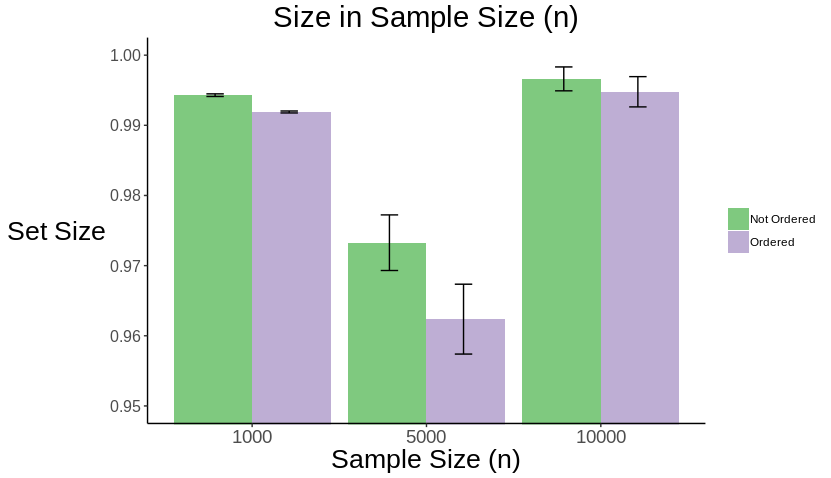
\includegraphics[scale=0.625]{images/Barplots/N_Size.png}
\caption{Sample Size (n) and Size}
\label{fig: Ordered_Size}
\end{figure}



\begin{figure}[H]
\centering
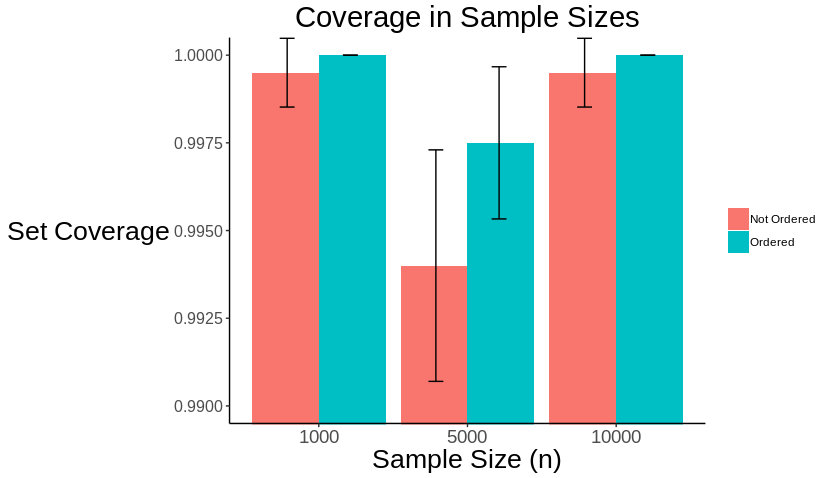
\includegraphics[scale=0.625]{images/Barplots/N_Cov.png}
\caption{Sample Size (n) and Coverage}
\label{fig: N_Cov}
\end{figure}


\section{Relationships to Disorder}
Now that relationships between disorder and size and disorder and coverage have been shown in certain scenarios, we wish to analyse overall trends.

To analyse overall trends, we simulated scenarios with varying values for covariates threshold, sample size, and odds ratio. This was done using the code described in \ref{Wrapper2}. The size and the coverage of the credible set is recorded for each simulation. 1000 credible sets were created, 5 rows of example data from is shown below in \ref{Sample Data_Cov Dis}. These data were used to analyse the relationships between a) -sum(log(pp)) and size b) -sum(log(pp)) and coverage. 



%sample data table 
\begin{table}[H] \centering 
  \caption{Sample Data} 
  \label{Sample Data_Cov Dis} 
\begin{tabular}{@{\extracolsep{5pt}} cccccccc} 
\\[-1.8ex]\hline 
\hline \\[-1.8ex] 
Ordered & Thr & Size & Number of Variants & Covered & Disorder & N & OR \\
\hline \\[-1.8ex] 
TRUE & $0.500$ & $0.508$ & $29$ & $0$ & $92.758$ & $5,000$ & $1.050$ \\ 
TRUE & $0.500$ & $0.799$ & $1$ & $1$ & $133.538$ & $2,000$ & $1.300$ \\ 
TRUE & $0.500$ & $0.506$ & $15$ & $1$ & $104.670$ & $4,000$ & $1.100$ \\ 
TRUE & $0.500$ & $0.504$ & $21$ & $1$ & $108.682$ & $5,000$ & $1$ \\ 
TRUE & $0.500$ & $0.509$ & $19$ & $0$ & $115.005$ & $5,000$ & $1.100$ \\ 
\hline \\[-1.8ex] 
\end{tabular} 
\end{table} 

Simulations were run 100, 500, and 1000 times comparing graphs and outputs. Logistic regression outputs for 1000 simulations are stated in this chapter, while regression outputs for 100 and 500 simulations can be found in the appendix. 



\section{Size and System Disorder} \label{System Disorder and Coverage}
The relationship between credible set size and disorder was explored. In %\ref{fig}
we can see that in the not ordered sets the number of variants in the credible set, size, is not effectively reduced. Disorder remains constant whether the sets are ordered or not ordered. We can see proof of this, as the disorder coefficient and variance is similar at 100 simulations and the same by 500 simulations. 

\subsection{Size Model }
%PUT TABLE FOR 1-4 MODELS






\subsection{Visualising Simulation Variability}
Plots shown 
%PUT ALL 3 GRAPHS HERE 

\begin{figure}[H]
    \caption {Size and Disorder in Varying Number of Simulations}    
    \begin{subfigure}[H]{\textwidth}
        \centering
        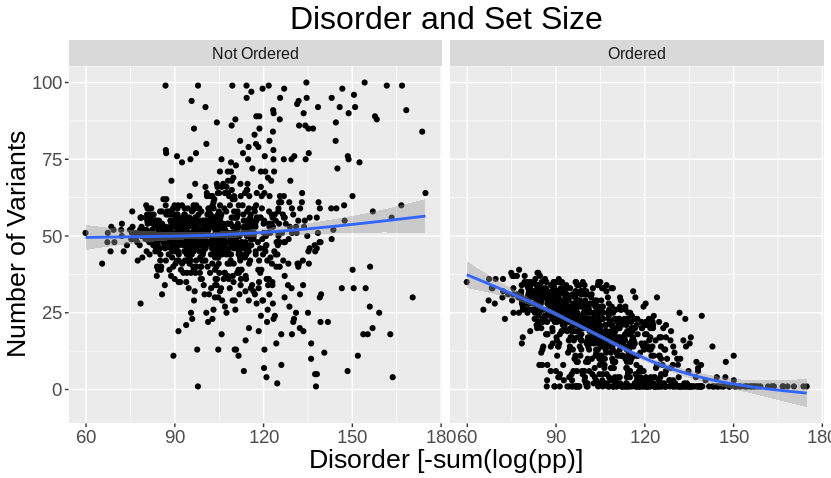
\includegraphics[width=\textwidth]{images/Size_and_Disorder_Charts/100_sim.png}
        \caption{100 Simulations}
        \label{}
    \end{subfigure}
    \hfill
    
    
    \begin{subfigure}[H]{\textwidth}
        \centering
        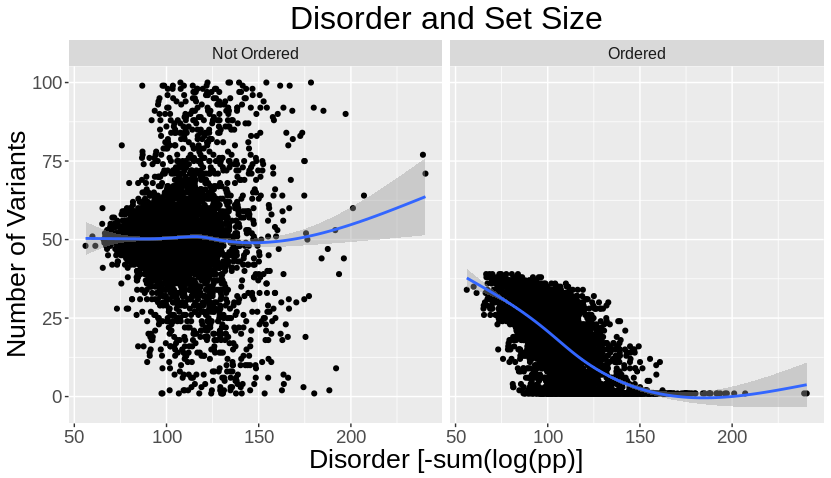
\includegraphics[width=\textwidth]{images/Size_and_Disorder_Charts/500_sim.png}
        \caption{500 Simulations}
        \label{}
    \end{subfigure}
    
\end{figure}
    
    
\begin{figure} \ContinuedFloat
    \centering
    \begin{subfigure}[]{\textwidth}
        \centering
        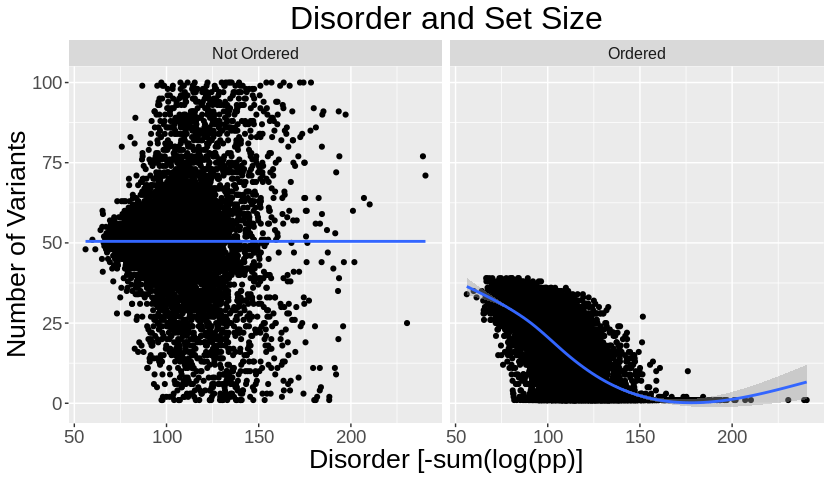
\includegraphics[width=\textwidth]{images/Size_and_Disorder_Charts/1000_sim.png}
        \caption{1000 Simulations}
        \label{}
    \end{subfigure}
    \label{}
\footnotesize
Values created for number of variants and disorder used covariate values of OR=1.5, Thr=0.5, 100 SNPs, and Sample size of 1000 cases and 1000 controls.
\end{figure}




\hl{The difference is how the trend changes in ordered versus not ordered sets. In not ordered sets, there is no general trend - indicated by the flat regression line.}

For the ordered sets, there is a downward trend, where as entropy increases, the size of the set gets smaller. This trend occurs because as entropy increases in ordered sets, we are increasing the the number of small p values - high association signals. This means we are also increasing the number of large posterior probabilities of the SNP being the causal variant. Very high disorder systems, as explored in \ref{Visualising Disorder in a Credible Set} have smaller sized sets, because the posterior probability one SNP is far greater than the other SNPs. Overall, the number of variants becomes smaller because we are considering less SNPs to be the causal variant. 


\section{Coverage and System Disorder} \label{Cov and Disorder}

\subsection{Model Selection - Akaike information criterion (AIC)}
The Akaike information criterion [@Akaike1974] was used to determine the best fit model for entropy. The model with the lowest AIC was selected as the best fit model. In this analysis different mathematical orders of entropy were analysed, first order = $x$, second order = $x^2$, third order = $x^3$, and fourth order $x^4$. The AIC is defined by:

\begin{equation}
\label{AIC}
{AIC}
 = -2k - 2log(\^L)
\end{equation}

The term $2k$ represents the number of parameters in the model and $-2log(\^L)$ represents how well the model explains the data. The goal of AIC is to give a \emph{relative} measure of model comparison. AIC penalises complex models by 1) $2k$ where more parameters, k, will increase the value of $2k$ and 2) $-log(\^L)$ where where the fit is worse, that is the likelihood estimate $(\^L)$, is poor, $(\^L)$ increases. It is important to note that AIC is used to determine which model is the best fit when comparing other models. AIC does \emph{not} give an absolute measure of how well the model fits the data. To answer how well the mode fits the data, linear regression has been used for set size and logistic regression for set coverage.  

\subsection{Finding Relationship between Coverage and Disorder}
Now that disorder has been defined as -sum(log(pp)), what is of interest are: \emph{1) What is the relationship between coverage and disorder?} This is explored through analysing different functional orders of disorder [-sum(log(pp))] and the AIC. \emph{2) Is there evidence against the hypothesis the relationship between coverage and disorder has no association?} In other words, is there a statistically significant relationship between coverage and disorder? This is investigated through logistic regression. 


%%AIC COV ORD
\begin{table}[H] \centering 
  \caption{Selecting Coverage Model (Orders Analysis) } 
  \label{Coverage Models} 
\begin{tabular}{@{\extracolsep{5pt}} ccccc} 
\\[-1.8ex]\hline 
\hline \\[-1.8ex] 
& equation & df & Ordered AIC & Not Ordered AIC \\ 
\hline \\[-1.8ex] 
First Order & $x$ & $2$ & $13,663.19$ & $13469.43$\\ 
Second Order & $x+x^2$ & $3$ & $13,586.74$ & $13428.01$\\ 
Third Order & $x+x^2+x^3$ & $4$ & $13,588.56$ & $13430.00$\\ 
Fourth Order & $x+x^2+x^3+x^4$ & $5$ & $13,590.46$ & $13431.98$\\ 
\hline \\[-1.8ex] 
\end{tabular} \\
  \smallskip
\footnotesize
AIC calculated under covariate values of: 1000 simulations, threshold of 0.9, odds ratio of 1.5, and sample size of 1000 cases and 1000 controls.
\end{table} 


For both ordered and not ordered sets, the second order equation had the lowest AIC values and were selected. The logistic regression model outputs from the second order equations are: 

%%LOG REG COV ORD TABLE 


\begin{table}[H] \centering 
  \caption{\textbf{Not Ordered} Sets: Coverage vs. Disorder Logistic Regression} 
  \label{Logistic Regression - Ordered Set Coverage} 
\begin{tabular}{@{\extracolsep{5pt}} ccccc} 
\\[-1.8ex]\hline 
\hline \\[-1.8ex] 
Coefficient & Estimate & Std. Error & z value & p-value \\ 
\hline \\[-1.8ex] 
Intercept & $0.27797$ & $0.02075$ & $13.396$ & $2e\mbox{-}16$ \\ 
Disorder & $38.10816$ & $2.61498$ & $14.573$ & $2e\mbox{-}16$ \\ 
Disorder$^2$ & $19.22267$ & $3.15373$ & $6.095$ & $1.09e\mbox{-}9$\\
\hline \\[-1.8ex] 
\end{tabular} \\
\smallskip
\footnotesize
Logistic regression statistics calculated under covariate values of: 1000 simulations, threshold of 0.5, odds ratio of 1.5, sample size of 1000 cases and 1000 controls, in \textbf{not ordered} sets. 
\end{table} 

\begin{table}[H] \centering 
  \caption{\textbf{Ordered} Sets: Coverage vs. Disorder Logistic Regression} 
  \label{Logistic Regression - Ordered Set Coverage} 
\begin{tabular}{@{\extracolsep{5pt}} ccccc} 
\\[-1.8ex]\hline 
\hline \\[-1.8ex] 
Coefficient & Estimate & Std. Error & z value & p-value \\ 
\hline \\[-1.8ex] 
Intercept & $0.5283$ & $0.02051$ & $2.576$ & $0.00999$ \\ 
Disorder & $35.65281$ & $2.53349$ & $14.073$ & $2e\mbox{-}16$ \\ 
Disorder$^2$ & $25.11611$ & $3.10983$ & $8.076$ & $6.67e\mbox{-}16$\\
\hline \\[-1.8ex] 
\end{tabular} \\
\smallskip
\footnotesize
Logistic regression statistics calculated under covariate values of: 1000 simulations, threshold of 0.9, odds ratio of 1.5, sample size of 1000 cases and 1000 controls, in \textbf{ordered} sets. 
\end{table} 



\section{Relationship between Number of SNPs and Disorder}
Before analysing how changing the number of SNPs effects coverage when we account for disorder, we first need to know how changing the number of SNPs effected disorder. Notice the change in x axis scale of entropy as more SNPs are considered.  

\begin{figure}[H]{\textwidth}
    \centering
    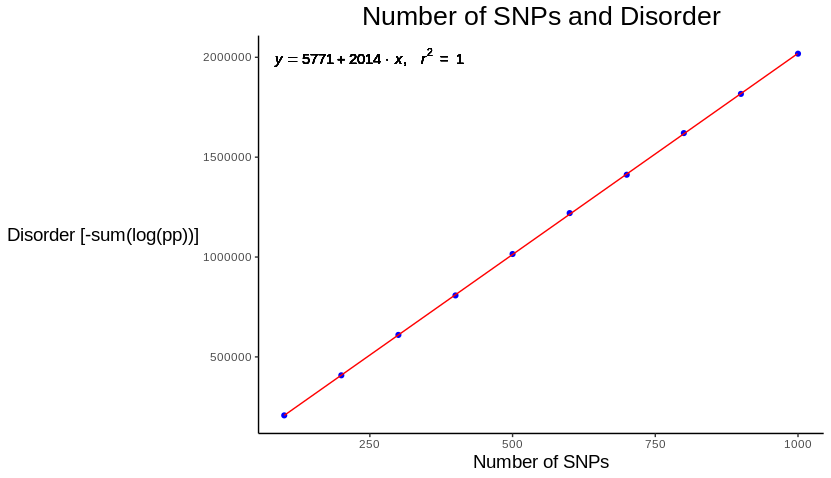
\includegraphics[width=\textwidth]{images/NumSNPs_vs_Disorder.png}
    \caption{Number of SNPs and Disorder}
    \label{fig:my_label}
    \footnotesize
Disorder computed from covariate values of simulations=100, OR=1.5, Thr=0.9, sample size of 1000 cases and 1000 controls. 
\end{figure}






\subsubsection{Simulation Data}
To determine this relationship simulations were run for 100-1000 SNPs. Covariate values were: Simulations= 100, Sample Size = 1000 cases and 1000 controls, OR=1.5, and  Threshold=0.9. Additionally, the sum disorder value for 1000 simulations with 1000 SNPs was validated to be $20,150,031.0$, which is ten times that of 100 simulations for 1000 SNPs as expected and maintains the linear property shown here. 

Simulation haplotype data ("artificial" LD matrix) showed a linear trend between SNPs and disorder. The error in the linear model is very low and due to simulation variation. 

\subsubsection{Issues with Simulation Data}
A couple issues emerge with utilising simulation data to find the relationship between increasing number of SNPs and entropy. The first is that the simulated haplotypes that create the LD matrix is artificial due to a 


\subsubsection{Real World LD - CLA4}
%DESCRIBE DATA/LD MATRIX
 
\section{Changing Number of SNPs Analysed} 
The same analysis was run for disorder and coverage, but looking at increasing SNP values. 
Values analysed were 100, 500, and 1000 SNPs.

Here we are showing that as -sum(log(pp))  increases, the coverage increases. 

The analysis shows that -sum(log(pp) is important and useful to capture, because it helps improve coverage – we are better able to make accurate claims for coverage of specified intervals. 

\subsection{100 SNPs}


\begin{figure}[H]
    \begin{centering}
    \caption{Coverage and Disorder in 100 SNPs}
    \begin{subfigure}[H]{\textwidth}
        \centering
        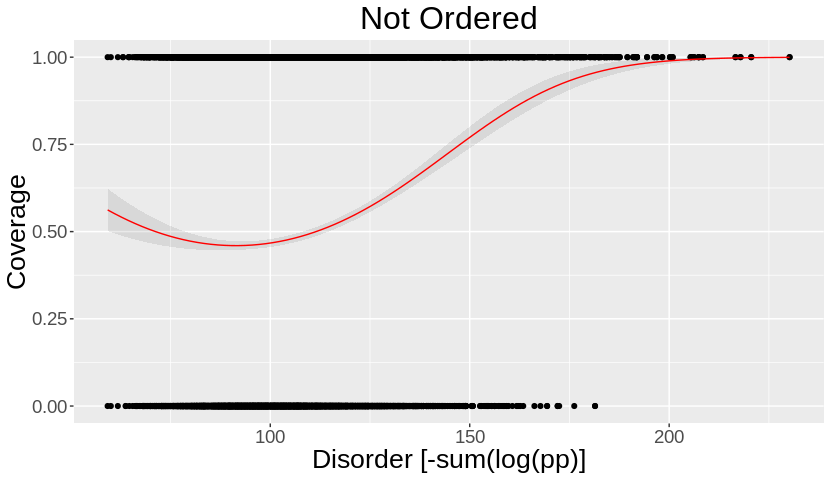
\includegraphics[width=\textwidth]{images/Coverage_and_Disorder_Charts/NotOrd_Cov_100SNPs.png}
        \caption{100 SNPs Not Ordered - 2nd Order Model}
        \label{}
    \end{subfigure}
    \hfill
    
    
    \begin{subfigure}[H]{\textwidth}
        \centering
        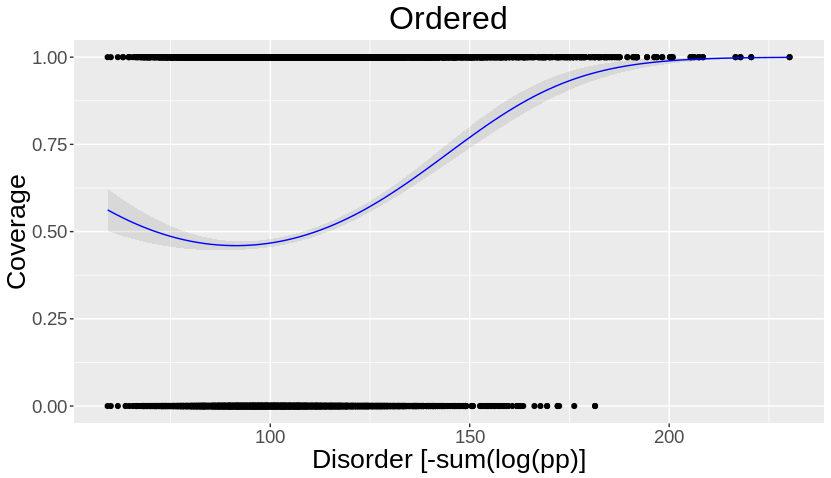
\includegraphics[width=\textwidth]{images/Coverage_and_Disorder_Charts/Ord_Cov_100SNPs.png}
        \caption{100 SNPs Ordered - 2nd Order Model}
        \label{}
    \end{subfigure}
    \label{}
\footnotesize
Plotter function was used to correct distribution. This adjusted predictions specified asymptotes to be within real world bounds of coverage between 0 and 1. Covariate values of: \textbf{500 SNPs}, 1000 simulations, threshold of 0.9, odds ratio of 1.5, sample size of 1000 cases and 1000 controls.
\end{centering}
\end{figure}


\subsection{500 SNPs}
\begin{figure}[H]
    \begin{centering}
    \caption {Coverage and Disorder 500 SNPs}
    \begin{subfigure}[H]{\textwidth}
        \centering
        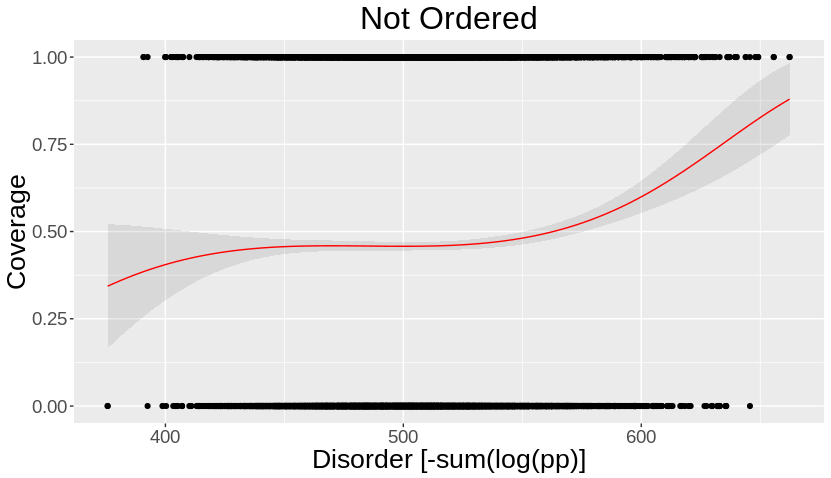
\includegraphics[width=\textwidth]{images/Coverage_and_Disorder_Charts/NotOrd_500SNPs.png}
        \caption{500 SNPs Not Ordered - 3rd Order Model}
        \label{}
    \end{subfigure}
    \hfill
    
    
    \begin{subfigure}[H]{\textwidth}
        \centering
        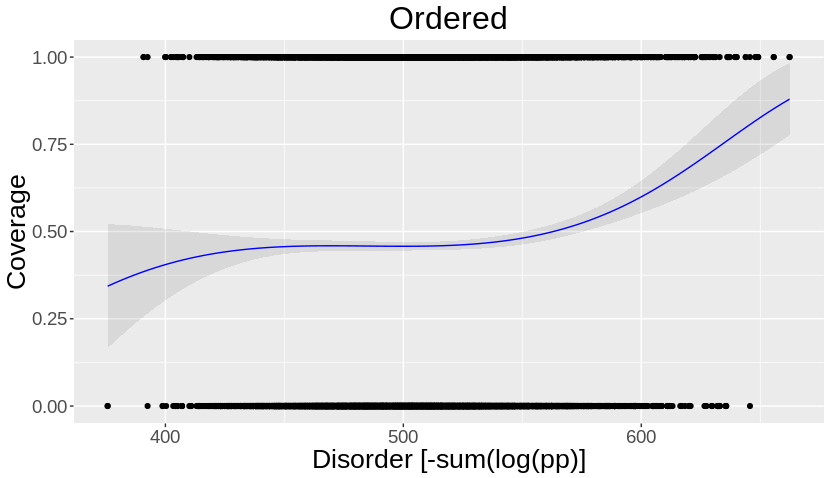
\includegraphics[width=\textwidth]{images/Coverage_and_Disorder_Charts/Ord_500SNPs.png}
        \caption{500 SNPs Ordered - 2nd Order Model}
        \label{}
    \end{subfigure}
    \label{}
\footnotesize
Plotter function was used to correct distribution. This adjusted predictions specified asymptotes to be within real world bounds of coverage between 0 and 1. Covariate values of: \textbf{500 SNPs}, 1000 simulations, threshold of 0.9, odds ratio of 1.5, and sample size of 1000 cases and 1000 controls.
\end{centering}
\end{figure}

\subsection{1000 SNPs}
\begin{figure}[H]
    \begin{centering}
    \caption {Coverage and Disorder 1000 SNPs}    \begin{subfigure}[H]{\textwidth}
        \centering
        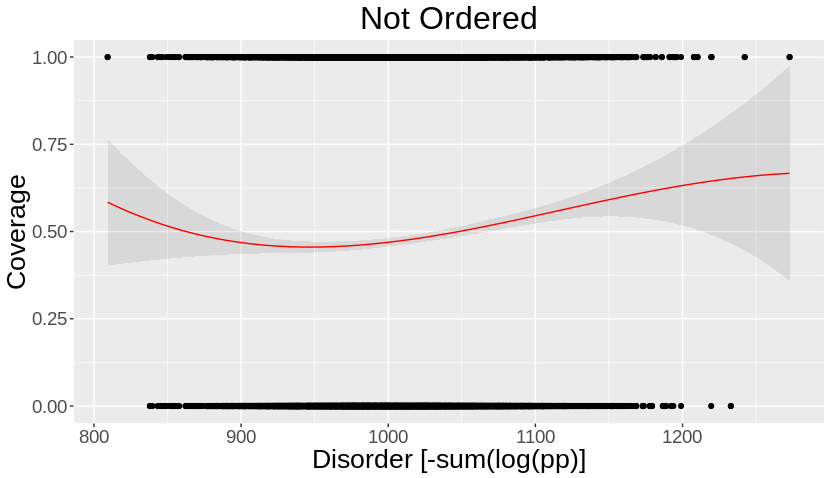
\includegraphics[width=\textwidth]{images/Coverage_and_Disorder_Charts/1000SNPs_3rdOrder_NotOrd.png}
        \caption{1000 SNPs Not Ordered - 3rd Order Model}
        \label{}
    \end{subfigure}
    \hfill
    
    
    \begin{subfigure}[H]{\textwidth}
        \centering
        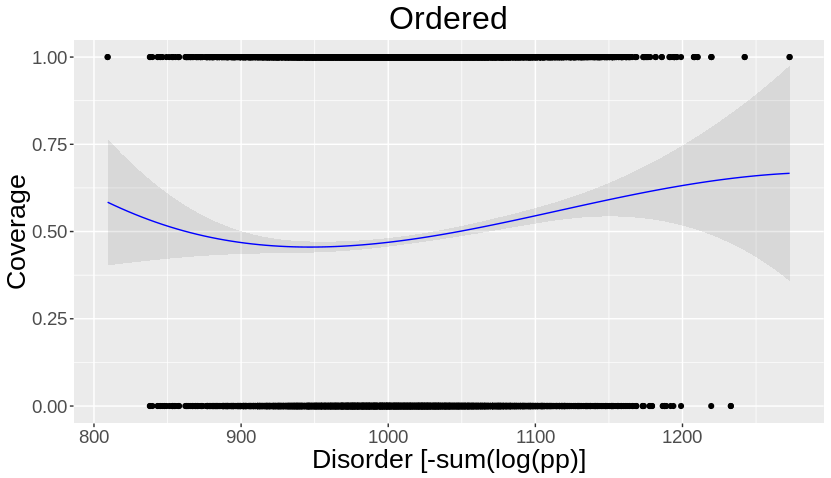
\includegraphics[width=\textwidth]{images/Coverage_and_Disorder_Charts/1000SNPs_3rdOrder_Ord.png}
        \caption{1000 SNPs  Ordered - 3rd Order Model}
        \label{}
    \end{subfigure}
    \label{}
\footnotesize
Plotter function was used to correct distribution. This adjusted predictions specified asymptotes to be within real world bounds of coverage between 0 and 1. Covariate values of: \textbf{1000 SNPs}, 1000 simulations, threshold of 0.9, odds ratio of 1.5, and sample size of 1000 cases and 1000 controls.
\end{centering}
\end{figure}

\pagebreak

\subsection{Quantifying Number of SNPs and Disorder}
By examining the figures that looked at 100, 500, and 1000 SNPs, we notice that the turning point - the point where the  derivative sign changes, is different in all figures. Each 

The trend across increasing number of SNPs and disorder was \emph{not constant}. The variation present means that how disorder contributes information about coverage depends on how many SNPs are being analysed. 







\section{Changing LD Strength and Disorder}
LD strength was analysed by utilising the original simulation data, where LD was "artificial" in that it had a specified lag sequence that created LD that had equal distance between high LD blocks and low LD hotspots 



\section{Changing Number of SNPs in LD}




%%Give regression output for set seed and no seed

\subsection{Set Seed Regression}

\subsection{No Seed Regression}


\section{Creating a Correction Factor for Credible Set }
fix!